\documentclass{article}

\usepackage{amsmath,graphicx,parskip,mathrsfs,subfigure}
\usepackage{fancyhdr}
\usepackage{amsthm,amssymb}
\usepackage{setspace}
\usepackage[left=3cm,right=3cm,top=3cm,bottom=3cm]{geometry}
%\usepackage{pslatex}
\pagestyle{fancy}
\lhead{Samuel Huberman}
\chead{ECE1336}
\rhead{999157923}

\newcommand{\unit}[1]{\ensuremath{\, \mathrm{#1}}}
\newtheorem{mydef}{Thereom}
\numberwithin{equation}{section}
\linespread{2.0}

\title{Thermal Conductivity from \textit{ab initio} Phonon Properties}
\date{December 12, 2011}
\author{Samuel Huberman ID:999157923}

\begin{document}

\maketitle
\newpage
\begin{spacing}{1.0}
\begin{tabular}{ l l }
  Nomenclature\\
  $a$ & Lattice constant \\
  $BE$ & Bose-Einstein distribution \\
  $c_v$ & Specific heat at constant volume, $J/K$\\
  $C_p$ & Volumetric specific heat at constant pressure, $J/m^3-K$\\
  $C_v$ & Specific heat at constant volume, $J/kg-K$\\
  $\textbf{e}$ & Normal mode polarization vector\\
  $E$ & Energy (kinetic and potential)\\
  $f$ & Phonon distribution function\\
  $\textbf{F}$ & Force vector (tensor)\\
  $\textbf{g}$ & Reciprocal space lattice vector\\
  $\mathscr{H}, H$ & Hamiltonian \\
  $\hbar$ & Planck's modified constant, 1.0546E-34 J-s\\
  $k_B$ & Boltzmann's constant, 1.3806E-23 J/K\\
  $k$ & Thermal conductivity\\
  $K$ & Spring constant\\
  $KE$ & Kinetic energy\\
  $\pmb{\kappa}$ & Phonon wavevector\\ 
  $\mathscr{L}$ & Lagrangian \\
  $m$ & Mass, constant\\
  $n$ & Electron density\\
  $N$ & Number of atoms\\
  $p$ & Probability distribution function, constant\\
  $\textbf{p}$ & Momentum vector\\
  $P$ & Pressure, function\\
  $\textbf{q},q$ & Heat flux vector, heat flux, charge\\
  $\vec{r},\textbf{r},r$ & Particle position, inter-particle separation\\
  $S$ & Normal mode coordinate\\
  $t$ & Time\\
  $T$ & Temperature\\
  $\textbf{u},u$ & Particle displacement from equilibrium\\
  $\textbf{v},v$ & Particle or phonon velocity\\
  $V$ & Potential or Volume\\
  $\pmb{\nu}$ & Phonon branch\\
  $\psi$ & Kohn-Sham orbitals\\
  $\epsilon$ & Kohn-Sham energy levels\\
\end{tabular}
\end{spacing}
\newpage
\section{Introduction}
Understanding thermal energy transport in light emitting diodes (LEDs) and photovoltaics is necessary to improve device performance. With a higher understanding of the dynamics of energy transfer at the nano-scale, we can begin the engineer solutions with specific applications in mind. Elucidating these dynamics begins with examining the behaviour of energy carriers: electrons and phonons. Here we focus upon the energy carried via phonons with the hope that in the future such knowledge of these two carriers and their interaction will lead to improved efficiencies in the aforementioned devices.\\

\section{Background}
The conventional approach used to examine heat conduction in solid relies upon the phenomenological Fourier's Law which states that the heat flux is directly proportional to the temperature gradient related by the material property of thermal conductivity.
\begin{align*}
		q=-k\frac{\partial T}{\partial x}
\end{align*}
Thermal conductivity, which is often assumed to be a constant in the application of Fourier's Law, is a function of temperature. This dependence can be accounted for by discretizing the domain with a finite element or finite difference method. However, the continuum picture begins to unravel when the solid of interest has a characteristic dimension that approaches the same order of magnitude as the mean free paths of the heat carriers. These heat carriers, which occur in any periodic solid regardless of its size, are referred to as phonons.

Often interpreted as quasi-particles representing the quantization of the kinetic energy of the lattice vibrations, phonons play an important role at the nanoscale because the average distance a given phonon may travel before an interaction is significantly affected by the size of the solid.

The dynamics of phonons has been extensively studied for the last century. With the increase in computational performance and the rise of nanotechnology, there has been a renewed interest in challenging task of simulating the dynamics of the quasi-particles. Naturally, in order to do so, a sufficient understanding of the fundamental physics is required.

Observable effects of these quantized energy carriers surround us. From the the insulation in our walls to the transistors of a CPU, the amount of heat that can be transferred through the solids depends upon the properties of phonons.

The importance of phonons can be illustrated through a series of examples. The original theory of high temperature superconductivity (BCS theory) indicated that phonons exerted themselves upon the electrons in such a way as to induce the generation of pair of electrons, known as a Cooper pairs, that would behave as particles with an integer spin and consequently reducing its tendency to interact with its surroundings. Although there is recent evidence that this is not the complete story of superconductivity [1], the less exotic behaviour of phonons cannot be ignored. Take a field effect transistor in a state where current can be transmitted. The heat sinks required to dissipate the energy from a CPU or GPU are a consequence of Joule heating, where some of kinetic energy of an electron under the presence of electric field is transmitted to the vibrational energy of the ions [2]. At the moment, Joule heating presents a challenge to chip manufacturers as the transistor size continues to shrink in accordance with Moore's law, without the generation of heat following suite. Recently, the strange quantum behaviour of entanglement has been experimentally produced within the vibrational state of two separated diamonds [3]. This result has potential applications towards quantum computing.

\section{Experiment}

Phonons can be observed experimentally through Neutron Scattering and Raman Spectroscopy [4]. The former technique, pioneered at Chalk River, Ontario by B.N. Brockhouse (who later received the Nobel Prize for this work), relies upon neutrons of a specified energy to strike a sample and scatter [5]. The change in energy of the scattered neutrons from the initial energy of the incident neutrons corresponds to the excitation of a vibrational mode of the sample. Similarly, Raman Spectrospcopy makes use to the principle of conservation of energy, but instead of neutrons, light in the ultra-violet and visible range is scattered by the sample. This exchange of energy from the light, like neutron scattering, indicates the generation of a phonon matching the difference of incident and scattered light.

\begin{figure}[ht]
\centering
\subfigure[]{
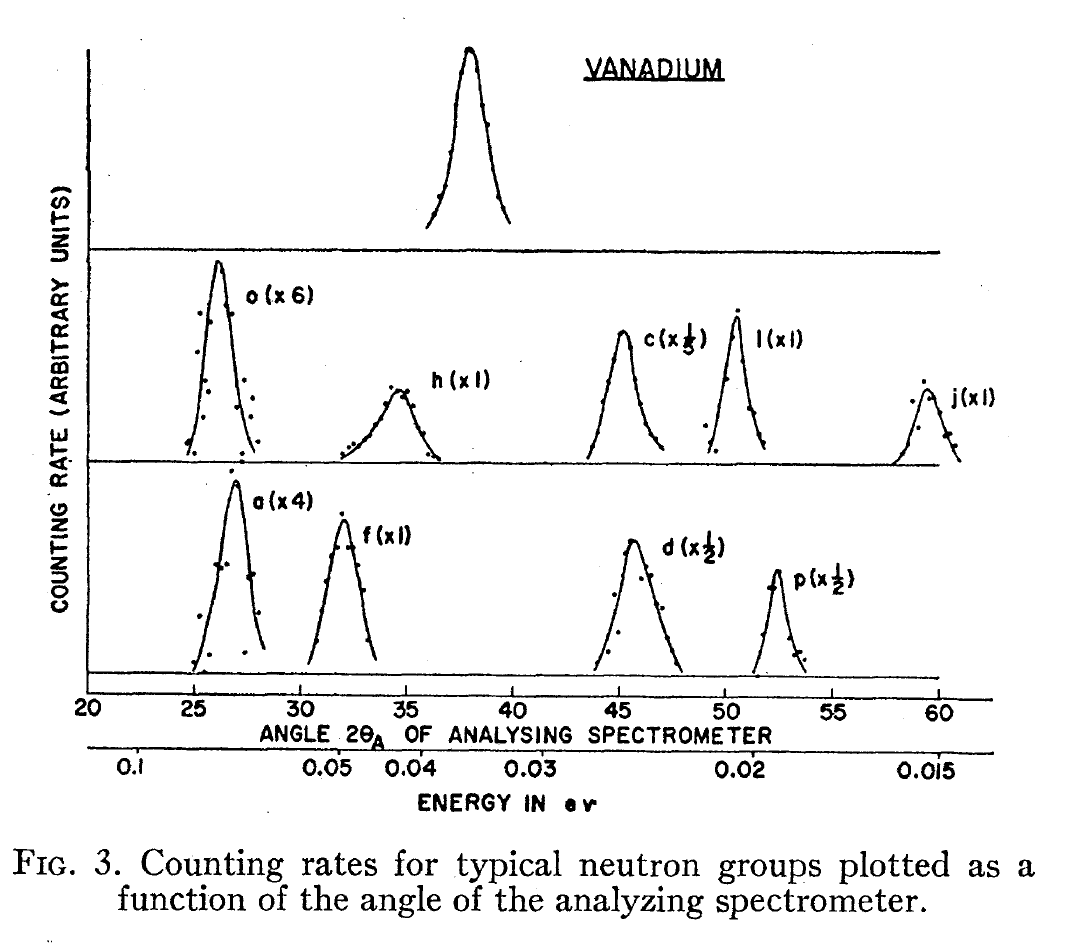
\includegraphics[scale=0.17]{neutron.png}
\label{fig:subfig1}
}
\subfigure[]{
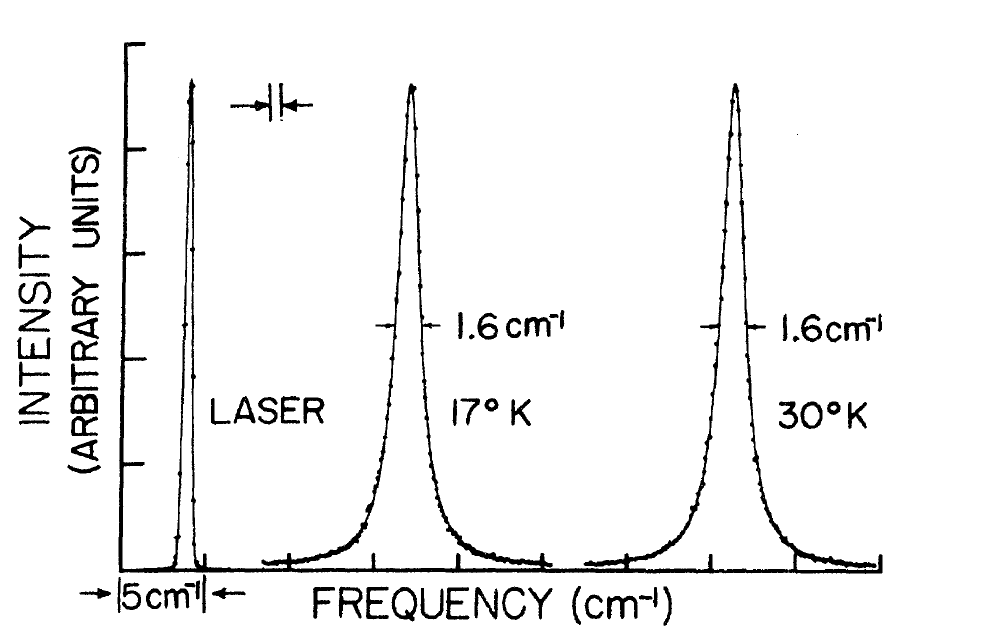
\includegraphics[scale=0.25]{raman.png}
\label{fig:subfig2}
}
\label{fig:subfigureExample}
\caption[Optional caption for list of figures]{(a) Experimental results from Neutron scattering displaying the intensity of scattered neutrons as a function of analyzing detector [5], (b) Experimental results from Raman Spectroscopy displaying the linewidth of the intensity peaks [6].}
\end{figure}

Probing solids with Neutron scattering and Raman Spectroscopy provides measureable insight into the properties of phonons [6]. By sending neutrons at different angles onto a sample, Brockhouse was able to construct dispersion curves. From Raman Spectroscopy, broadening of the intensity peaks with increasing sample temperature corresponds to a decrease in the time between phonon interactions. Through a theoretical examination, the importance of these properties will become clear.

\section{Theory}

Each phonon, corresponding to a normal mode of vibration of the lattice, is associated with three properties: the lifetime of its existence, the group velocity and the specific heat. The overall contribution of each phonon mode towards thermal conductivity relies upon the accurate prediction of these properties [7]:
\begin{align*}
	k= \sum_\nu\sum_\kappa c_{ph}(\pmb{\kappa},\nu)v^2_g(\pmb{\kappa}, \nu)\tau_{p-p}(\pmb{\kappa}, \nu)
\end{align*}
As a starting point, the dynamics of simplified model of a one dimensional linear chain of atoms are reviewed. The model is then extended to a proper three-dimensional lattice. Finally, the challenge of determining the lifetime of a phonon mode and its inclusion into a phonon transport model is discussed.

\subsection{Introduction to Lattice Dynamics}
\begin{figure}[ht]
\centering
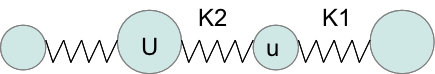
\includegraphics[scale=0.5]{diatomic.png}
\caption{Diagram of a linear diatomic chain of atoms}
\end{figure}
Recalling the equations of motion of a linear diatomic chain considering only nearest neighbour interaction ($K_1$ and $K_2$ are the respective spring constants in accordance with Hooke's Law) [8]:
\begin{align*}
	M\frac{\partial ^2 u_n}{\partial t^2}&=-K_1(U_n-u_n)-K_2(U_n-u_{n-1})\\
	m\frac{\partial ^2 u_n}{\partial t^2}&=-K_1(u_n-U_n)-K_2(u_n-U_{n+1})
\end{align*}
Recognizing that the solutions to the equations will have the periodic form:
\begin{align*}
	U_n&=\sum_\kappa \tilde{U_\kappa}e^{i(\kappa na-\omega t)}\\
	u_n&=\sum_\kappa \tilde{u_\kappa}e^{i(\kappa na-\omega t)}
\end{align*}
Upon the application of the proper boundary conditions (the Born-von Karman periodic boundary, where the last atom in the chain is equivalent to the first in the chain), a discrete set of allowed values of $\kappa$ emerges (this condition is not affected by the fact that the masses of the chain alternate):
\begin{align*}
	\pmb{\kappa}=\frac{2\pi m}{Na}
\end{align*}
Each $\kappa$ in this set corresponds to a different phonon mode. The two coupled ordinary differential equations can be represented in terms of an eigenvalue problem:
\[
\begin{bmatrix}
  -M\omega_\kappa^2 & 0\\
  0 & -m\omega_\kappa^2\\ 
 \end{bmatrix}
\begin{bmatrix}
\tilde{U_\kappa} \\ 
\tilde{u_\kappa}
\end{bmatrix}
=
\begin{bmatrix}
  -(K_1+K_2) & K_1+K_2e^{-i\kappa a}\\
  -(K_1+K_2) & K_1+K_2e^{-i\kappa a}\\ 
 \end{bmatrix}
\begin{bmatrix}
\tilde{U_\kappa} \\ \tilde{U_\kappa}
\end{bmatrix}
\]
The eigenvalues are the allowed frequencies and the eigenvectors are the allowed amplitudes for a given value of $\pmb{\kappa}$. The range of wavevectors, which operate in reciprocal space,  $\frac{-\pi}{a}\leq \pmb{\kappa}\leq\frac{\pi}{a}$ gives the first Brillouin zone. Because of the periodic nature of the lattice and hence $\pmb{\kappa}$, values outside this region may be folded back over so as to be included in the first Brillouin zone.

Applying this approach to a genuine lattice structure requires information about the interatomic potentials. For silicon, the empirical Stilinger-Weber potential is typically used in molecular dynamic simulations [7]. For rare gas solids like argon, the Lennard-Jones potential describes the interatomic energy [8]:
\begin{align*}
	\phi(r)=-4\epsilon[(\frac{\sigma}{r})^6-(\frac{\sigma}{r})^{12}]	
\end{align*}
The spring constants in the equations of motions of the atoms of the lattice can then be calculated by expanding the energy of the lattice in Taylor series:
\begin{align*}
	E&=N\phi(a)\\
	E&=N\phi+\sum_{s\geq1}\frac{1}{s!}\frac{\partial^s\phi}{\partial u^s}\sum_n(u_n-u_{n+1})^s
\end{align*}
The harmonic approximation is the truncation of this expansion, neglecting orders greater than two. From this expansion, we find that the force constants must be:
\begin{align*}
%	m\frac{\partial ^2 u_n}{\partial t^2}&=\frac{-\partial E_{harmonic}}{\partial u_n}=-\frac{\partial^2 E}{\partial u_n\partial u_{n+1}}(2u_n-u_{n+1}-u_{n-1})\\
	K_1&=\frac{\partial^2 E}{\partial u_n\partial U_{n}}\\
	K_2&=\frac{\partial^2 E}{\partial u_n\partial U_{n+1}}
\end{align*}
Under this approximation, the force acting on atom $a$ as a result of displacement of atom $b$ in the unit cell is the second derivative of the potential with respect to the displacement of both atoms. This definition extends to three dimensional structures by including the direction of the displacement and the force.
\[ 
\Phi_{ab}=
\begin{bmatrix}
  \frac{\partial^2 \phi}{\partial u^a_i\partial u^b_i} & \frac{\partial^2 \phi}{\partial u^a_i\partial u^b_j} &\frac{\partial^2 \phi}{\partial u^a_i\partial u^b_k}\\
  \frac{\partial^2 \phi}{\partial u^a_j\partial u^b_i} & \frac{\partial^2 \phi}{\partial u^a_j\partial u^b_j} &\frac{\partial^2 \phi}{\partial u^a_j\partial u^b_k}\\
\frac{\partial^2 \phi}{\partial u^a_k\partial u^b_i} & \frac{\partial^2 \phi}{\partial u^a_k\partial u^b_j} &\frac{\partial^2 \phi}{\partial u^a_k\partial u^b_k}
 \end{bmatrix}
\]
Provided with the knowledge of these harmonic force constants, the general form of the eigenvalue problem is then constructed [8]:
\begin{align*}
	\omega^2(\pmb{\kappa},\nu) e(\pmb{\kappa},\nu)=D(\pmb{\kappa})e(\pmb{\kappa},\nu) 
\end{align*}
The dynamical matrix, $D(\pmb{\kappa})$ contains the chunks of 3 by 3 force constants from $\Phi_{ab}$ as well as the time independent portion of the general solution form and as such depends upon the wavevector. Solving this matrix equation over a grid of wavevectors in the first Brillouin zone, provides a set of data where frequency is a function of wavector known formerly as dispersion relations (unlike the diatomic case, there more than two possible branches, $\nu$, as a result of the greater number of degrees of freedom of the atoms in the unit cell). From which, we can find two phonon properties, the group velocity of each phonon mode [7]:
\begin{align*}
v_g(\pmb{\kappa}, \nu)=\frac{\partial \omega(\pmb{\kappa},\nu)}{\partial \pmb{\kappa}}
\end{align*}
And the specific heat of each phonon from the classical thermodynamic definition [7]:  
\begin{align*}
c_{ph}(\pmb{\kappa},\nu)=\frac{\partial E}{V\partial T}=\frac{\hbar\omega(\pmb{\kappa},\nu)}{V}\frac{\partial f^{BE}(\pmb{\kappa}, \nu)}{\partial T}	
\end{align*}
 
\subsection{Phonon gas picture}
Once we have obtained the set of possible normal modes of for a given material, the dynamics of phonons can now be probed. The statistical nature of the large number of phonons makes use of extending the analogy of the transport behaviour of gas particles. The change in the distribution of the phonons over time is determined by the the Boltzmann Transport Equation (BTE):
\begin{align*}
	\frac{\partial f(\pmb{\kappa}, \nu)}{\partial t}+v_g(\pmb{\kappa}, \nu)\cdot\nabla f(\pmb{\kappa}, \nu)= [\frac{\partial f(\pmb{\kappa}, \nu)}{\partial t}]_{coll}
\end{align*}
However, unlike the standard gas BTE, the phonon BTE exists for every possibly phonon mode. Difficulties in solving the BTE are primarily to due the challenge of accurately representing the collision term. A common approach is to linearize this term, which is known as the relaxation time approximation:
\begin{align*}
	\frac{\partial f(\pmb{\kappa}, \nu)}{\partial t}+v_g(\pmb{\kappa}, \nu)\cdot\nabla f(\pmb{\kappa}, \nu)= \frac{f^{BE}(\pmb{\kappa}, \nu)-f(\pmb{\kappa}, \nu)}{\tau(\pmb{\kappa}, \nu)}
\end{align*}
Accordingly, $\tau$ is defined as the average time a given phonon mode travels unimpeded before interacting (colliding in the particle picture) with a boundary, an electron or another phonon. The Matthiesen rule combines these processes like the circuit equivalent of resistors in parallel [7]:
\begin{align*}
\frac{1}{\tau(\pmb{\kappa}, \nu,L)}&=\frac{1}{\tau_{p-p}(\pmb{\kappa}, \nu)}+\frac{1}{\tau_{b}(\pmb{\kappa}, \nu,L)}+\frac{1}{\tau_{p-e}(\pmb{\kappa},\nu)}\\
\tau_{b}(\pmb{\kappa}, \nu,L)&=\frac{L/2}{|v_g(\pmb{\kappa}, \nu)|}\\
\frac{1}{\tau_{p-e}}&=\frac{n_e\epsilon_1^2\omega}{\rho V_g^2k_BT}\sqrt{\frac{\pi m^{*}V_g^2}{2k_BT}}exp(-\frac{m^{*}V_g^2}{2k_BT})
\end{align*}
At this point it is assumed that the phonon-electron,$\tau_{p-e}$, and boundary interaction,$\tau_{b}(\pmb{\kappa}, \nu,L)$, can be calculated from the above formulas. However, a thorough investigation is required in order to assess their applicability under different conditions. Such effort is outside the scope of this work. 

\subsection{The details of $\tau$}
The simplicity of the lattice dynamics approach relied upon the validity of the harmonic approximation. At low temperatures (where the atoms vibrations about equilibrium are small such that $u<<a$), such an approximation offers a solid step towards estimating group velocity and specific heat. However, the phenomena of thermal expansion and the finite thermal conductivity of a lattice will not appear in this picture because of the neglect of the anharmonic terms in the energy expansion (or equivalently the lattice Hamiltonian). These anharmonic terms are responsible for phonon-phonon interaction.

Interaction here is the transition of a phonon from one mode to another. As such, the principles of conservation of energy and the interference condition for wavevectors are required, imposing what are known as selection rules [9]:
\begin{align*}
	\hbar\omega(\pmb{\kappa},\nu)+\hbar\omega(\pmb{\kappa}',\nu')&=\hbar\omega(\pmb{\kappa}'',\nu'')\\
	\pmb{\kappa}+\pmb{\kappa'}=\pmb{\kappa''}+\pmb{g}
\end{align*}
From these relations, the outcome of a phonon of mode $(\pmb{\kappa},\nu)$ interacting with another mode $(\pmb{\kappa'},\nu')$ is to combine to create a mode $(\pmb{\kappa}'',\nu'')$. The reverse is also true: a mode $(\pmb{\kappa}'',\nu'')$ can split into two phonons of modes $(\pmb{\kappa},\nu)$ and $(\pmb{\kappa'},\nu')$. These are known as three phonon processes, of which there are two types: Normal and Umklapp. The former being the case of $\pmb{g}=0$ (the integer factor of the lattice vector being zero), indicating the conservation of momentum while the latter occurs when in $\pmb{g}\neq 0$ (the integer factor of the lattice vector being non-zero). At this point an interesting note is worth making: in the phonon field picture, the operator of each phonon mode has an expectation value of zero and consequently there is no transfer of momentum in a lattice vibration [9].

In accordance with the selection rules of phonon-phonon interaction, time between these transitions can now be probed. Relying upon the results of time-dependent perturbation theory, the probability of a transition from one state to another is given by Fermi's Golden rule [9]:
\begin{align*}
P_{i-f}=\frac{2\pi}{\hbar}|\langle i|\mathscr{H}'|f\rangle|^2 D_f(\epsilon_i)
\end{align*}
Thus, the probability of a transition from state $|i\rangle$ to $|f\rangle$ is proportional to the square of the matrix element of the perturbed Hamiltonian weighted by the number of final states with energy $\epsilon_i$. Here, the perturbed Hamiltonian corresponds to the higher order terms in the Taylor energy expansion. Through some algebraic manipulation of Fermi's Golden rule using the probability of transition per unit of time and ignoring terms of degree greater than three, the significant result can be succinctly represented [13]:
\begin{align*}
\tau_{p-p}(\pmb{\kappa},\nu)\propto (\frac{\partial^3 E}{\partial u^a_i(\pmb{\kappa},\nu)\partial u^b_i(\pmb{\kappa'},\nu')\partial u^c_k(\pmb{\kappa''},\nu'')})^{-1}
\end{align*}
The final missing phonon property requires the determination of the third derivative of energy with respect to the respective atoms' displacements. Like the 3 by 3 matrix of the harmonic force constants for a given pair of atoms, the cubic force constant form a 3 by 3 by 3 tensor for triplet of atoms.  The task is now to accurately extract these cubic force constants.

\subsection{Introduction to Density Functional Theory}
 
The use of these empirical potentials leads to an inherent inaccuracy in the generated properties as information concerning the cubic force constants is not correctly encoded, thereby presenting the impetus of studying phonons from first principle methods. At the moment, the most popular approach is to use density functional theory (DFT) [10,11] to calculate the exact interatomic potential (and hence the required force constants), from which the phonon lifetimes can be extracted, exemplified through the work of Broido et al [12] and later Esfarjani et al [13].

The theoretical framework of DFT was first constructed by Walter Kohn (a University of Toronto alumn) as a workaround for solving the many-body problem in solid state physics. Relying upon the two theorems outlined below, Kohn was able to reduce the degrees of freedom in such a way that allows one to a solve single electron Schrodinger-like equation instead of facing the large number of dimensions in the many-body Schrodinger equation. \footnote{Under the Born-Oppenheimer approximation (or equivalently the adiabatic approximation), the nuclear and electronic degrees of freedom become decoupled. The electrons are hereby assumed to follow the motion of the atomic core without exchanging energy with its surroundings (equilibrium).}
\begin{mydef}The ground-state energy from Schrodinger's equation is a unique function of the electron density.
\end{mydef}
The electron density can be defined in terms of the individual electron wavefunctions:
\begin{align*}
	n(\vec{r})&=2\sum_i\psi_i^*(\vec{r})\psi_i(\vec{r})
\end{align*}
\begin{mydef}The electron density that minimizes the energy of the overall functional is the true electron density corresponding to the full solution of the Schrodinger equation.
\end{mydef}
The energy functional (a functional is a function of a function) is defined as:
\begin{align*}
	E[\psi]=E_{known}[\psi]+E_{XC}[\psi]
\end{align*}
The single electron Kohn-Sham equations have the form:
\begin{align*}
	[\frac{\hbar^2}{2m}\nabla^2+V(\vec{r})+V_H(\vec{r})+V_{XC}]\psi_i(\vec{r})=\epsilon_i\psi_i(\vec{r})
\end{align*}
$V(\vec{r})$ represents the interaction between the electron and the collection of nuclei:
\begin{align*}
	V(\vec{r})=V(\vec{r+a})
\end{align*}
$V_H(\vec{r})$, known as the Hartree protential, represents the Coulomb repulsion between the electron and the total electron density:
\begin{align*}
	V_H(\vec{r})=e^2\int\frac{n(\vec{r'})}{|\vec{r}-\vec{r'}|}d^3\vec{r'}
\end{align*}
Since the Hartree potential includes the electron's interaction with itself, the final term, the exchange-correlation potential, corrects this unphysical behaviour (More accurately, this potential describes the quantum mechanical property of indistinguishable particles. The exchange part refers to the energy change from a change in spatial coordinates, the correlation term refers to the fact the electrons are really electron densities):
\begin{align*}
	V_{XC}(\vec{r})=\frac{\delta E_{XC}(\vec{r})}{\delta n(\vec{r})}
\end{align*}
Presently, there does not exist an exact form for $E_{XC}$, so current implementations of DFT rely upon approximate forms of this term. The simplest approximation, called the local density approximation (LDA), describes the exchange-correlation potential to be that of the exchange-correlation potential of a uniform electron gas at the electron density observed at that position:
\begin{align*}
	V_{XC}(\vec{r})=V_{XC}^{electron gas}[n(\vec{r})]
\end{align*}
Once a representation of the exchange-correlation term has been chosen, an iterative approach to describing a self-consistent system is undertaken. A trial electron density is chosen to first solve the Kohn-Sham equations to find the single particle wave functions $\psi_i(\vec{r})$. A new electron density is then recalculated using these wave functions and compared to the initial electron density. This new electron density is then used in the Kohn-Sham equations and the procedure is repeated until convergence has been reached.

The obtained ground state energy is known as the adiabatic potential energy surface. This energy surface is a function of nuclear positions. One of the crucial advantages of DFT is the ease with which we can displace an ion from its equilibrium position and quickly recalculate the energy surface for this new configuration. Since the ion is no longer at equilibrium, there will be a force exerted upon it as well as neighbouring atoms. Through a series of systematic displacements and relying upon the crystal symmetry for simplification, a number of linear force-balance equation enables one to solve for the higher-order force constants [14]. An alternative is to regard the displacement as a small disturbance and apply perturbation theory to the Kohn-Sham equations (this approach is discussed in the appendix) [15,16]. 

\section{Results}
An attempt was made to numerically observe the bulk properties of phonons in silicon. Using a combination of the pw.x, ph.x and q2r.x codes offered in the QUANTUM-ESPRESSO package [17], the dispersion and the density of states was obtained. Alas, the cubic force constants remained elusive.

\begin{figure}[!ht]
\centering
\subfigure[]{
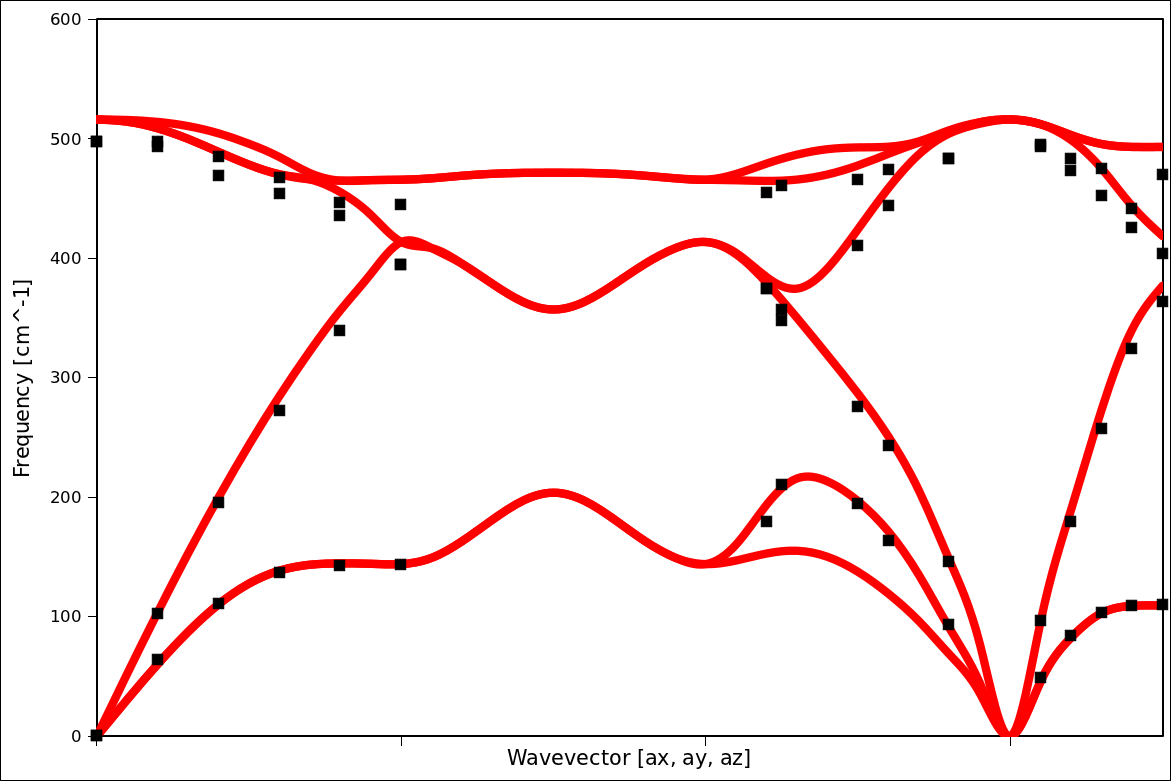
\includegraphics[scale=0.2]{dispersion1.png}
\label{fig:subfig1}
}
\subfigure[]{
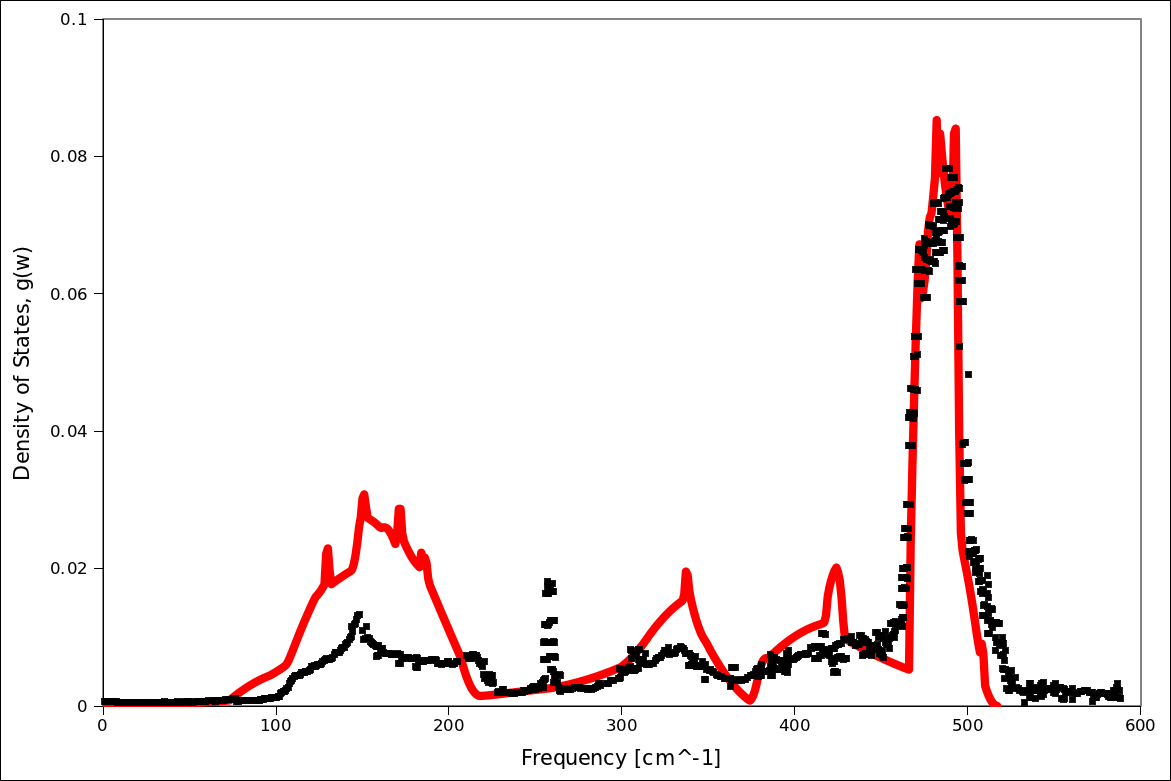
\includegraphics[scale=0.2]{dos1.png}
\label{fig:subfig2}
}
\label{fig:subfigureExample}
\caption[Optional caption for list of figures]{\subref{fig:subfig1} Dispersion of silicon from DFT calculations (line) and experimental data (square markers) at 300K from [18], \subref{fig:subfig2} Density of states from DFT calculations (line) and experimental data (square markers) at 305K from [6].}
\end{figure}
From both the dispersion and density of states plots, density functional theory provides excellent agreement with experimental data. The apparent vacancy of dispersion data is purely the result of no measurements being done in the corresponding directions of the Brillouin zone. Experimental data of the phonon-phonon lifetime remains scarce and appears to have only been tabulated for zone-center acoustic and optical [4].

\section{Conclusion}

In order to determine the effective thermal conductivity of nano-scale materials, the ability to predict the properties of phonons is necessary. As a simple first step, empirical potentials in combination with lattice dynamics calculations can be used to find dispersion relations and consequently the mode specific group velocity and specific heat. 

The prediction of the final property, the phonon-phonon lifetime, continues to present a challenge, though first principle methods like DFT have demonstrated some success on this front. Here, it was shown that DFT can be used to determine the bulk phonon properties of silicon. In the future, this approach can be used to determine the phonon properties of nano-scale systems, such as thin films. Combining the phonon properties extracted from DFT with the hierarchical approach outlined by Sellan, a complete picture of the thermal energy transfer in nano-structured systems can be constructed.

The determination of other the lifetimes of other phonon interactions, like boundary and electron scattering, are as important and deserve further attention. DFT can be used to probe the electron-phonon interaction but the periodic nature of the technique makes the study of interfaces difficult.
\newpage
\section{References}
\begin{spacing}{1.0}
\small
\noindent
[1] P. Monthoux, D, Pines, G.G. Lonzarich, Nature \textbf{450}, 1177 (2007).\newline
[2] E. Pop, ASME Conf. Proc. ENIC2008-53050, 129-132 (2008).\newline
[3] K. C. Lee et al. Science \textbf{334}, 1253 (2011).\newline
[4] A. Debernardi, ``Anharmonic Porperties of Semiconductors from Density-Functional Perturbation Theory", \textit{Thesis} (1995).\newline
[5] B. N. Brockhouse and P. K. Ivengar, Phys. Rev. \textbf{111}, 747 (1958).\newline
[6] P. A. Temple and C. E. Hathaway, Phys. Rev. B \textbf{7}, 3685 (1973).\newline
[7] D. P. Sellan, J. E. Turney, A. J. H. McGaughey and C. H. Amon, J. Appl. Phys. \textbf{108}, 113524 (2010).\newline
[8] M. T. Dove, \textit{Introduction to Lattice Dynamics}, Cambridge University Press (1993).\newline
[9] J. M. Ziman, \textit{Electrons and Phonons}, Oxford University Press (1960).\newline
[10] D. S. Sholl and J. A. Steckel, \textit{Density Functional Theory: A Practical Introduction}, Wiley, (2009).\newline
[11] P. Giannozzi, S. de Gironcoli, P. Pavone and S. Baroni, Phys. Rev. B. \textbf{43}, 7231 (1991).\newline
[12] D. A. Broido, M. Malorny, G. Birner, Natalio Mingo, and D. A. Stewart, Appl. Phys. Lett. \textbf{91}, 231922 (2007).\newline
[13] K. Esfarjani, G. Chen, Phys. Rev. B. \textbf{84}, 085204 (2011).\newline
[14] K. Esfarjani and H.T. Stokes, Phys. Rev. B. \textbf{77}, 144112 (2008).\newline
[15] S. Baroni, S. de Gironcoli, A. Dal Corso, and P. Giannozzi, Rev. Mod. Phys. \textbf{73}, 515 (2001).\newline
[16] X. Gonze and J.-P. Vigneron, Phys. Rev. B. \textbf{39}, 13120 (1989).\newline
[17] P. Giannozzi, S. Baroni, N. Bonini, M. Calandra, R. Car, C. Cavazzoni, D. Ceresoli, G. L. Chiarotti, M. Cococcioni, I. Dabo, A. Dal Corso, S. Fabris, G. Fratesi, S. de Gironcoli, R. Gebauer, U. Gerstmann, C. Gougoussis, A. Kokalj, M. Lazzeri, L. Martin-Samos, N. Marzari, F. Mauri, R. Mazzarello, S. Paolini, A. Pasquarello, L. Paulatto, C. Sbraccia, S. Scandolo, G. Sclauzero, A. P. Seitsonen, A. Smogunov, P. Umari, R. M. Wentzcovitch, J. Phys. Condens. Matter \textbf{21}, 395502 (2009).\newline
[18] G. Dolling in \textit{Inelastic Scattering of Neutrons in Solids and Liquids}, edited by S. Ekland (IAEA, Vienna, 1963), Vol. II p.37. \newline
%[ ] G. Nilsson and G. Nelin, Phys. Rev. B \textbf{3}, 364 (1971).\newline

\newpage
\section{Appendix}
\subsection*{Introduction to Density Functional Perturbation Theory}
First note, the Hellmann-Feynman theorem:
\begin{align*}
	H_{\lambda}\Psi_{\lambda}&=E_{\lambda}\Psi_{\lambda}\\
        \frac{\partial E_{\lambda}}{\partial \lambda}&=\langle \Psi_{\lambda}|\frac{\partial H_{\lambda}}{\partial \lambda}|\Psi_{\lambda}\rangle
\end{align*}

Like the application of perturbation theory to the Schroedinger Equation, the ionic potential acts as a perturbation:
\begin{align*}
        V_{SCF}(r)&->V_{SCF}(r)+\Delta V_{SCF}(r)\\
	V_{SCF}(r)&=V_{ion}(r)+e^2\int \frac{n(r')}{|r-r'|}dr'+v_{xc}(n(r))\\
	\Delta V_{SCF}(r)&=V_{bare}(r)+e^2\int \frac{\Delta n(r)n(r')}{|r-r'|}dr'+\Delta n(r)\frac{dv_{xc}}{dn}
\end{align*}
The perturbed Kohn-Sham:
\begin{align*}
	(H_{SCF}-\epsilon_n)\mid\Delta\psi_n\rangle&=-(\Delta V_{SCF}-\Delta \epsilon_n)\mid\Delta\psi_n\rangle
\end{align*}
Equivalently written:
\begin{align*}
	(H_{SCF}-\epsilon_n)\mid\frac{\partial \psi_n}{\partial \lambda}\rangle&=-(\frac{\partial V_{SCF}}{\partial \lambda}-\epsilon_n^{(1)})\mid\psi_n\rangle        
\end{align*}
Assuming the perturbation is reasonably small, the energy can be represented as a power series:
\begin{align*}
	H_{SCF}=H^{(0)}+\lambda H^{(1)}+\lambda^2 H^{(2)}+\lambda^3 H^{(3)}\\
        E=E^{(0)}+\lambda E^{(1)}+\lambda^2 E^{(2)}+\lambda^3 E^{(3)}
\end{align*}
The first and second derivatives (equivalently, the first and second order corrections to the energy):
\begin{align*}
E^{(1)}&=\frac{\partial E}{\partial \lambda_i}=\int \frac{\partial V_{\lambda}}{\partial \lambda_i}n_{\lambda}(\pmb{r})d\pmb{r}\\
E^{(2)}&=\frac{\partial^2 E}{\partial \lambda_i\partial \lambda_j}=\int \frac{\partial V^2_{\lambda}(\pmb{r})}{\partial \lambda_i\partial \lambda_j}n_{\lambda}(\pmb{r})dr+\int\frac{\partial V_{\lambda}(\pmb{r})}{\partial \lambda_j}\frac{\partial n_{\lambda}(\pmb{r})}{\partial \lambda_i}d\pmb{r}
\end{align*}
The third order derivatives [].:
\begin{align*}
E^{(3)}&=\frac{\partial^3 E}{\partial \lambda_i\partial \lambda_j\partial \lambda_k}&=6 \sum_v\langle\psi_v^{(1)}|H^{(1)}_{SCF}-\epsilon_v^{(1)}|\psi_v^{(1)}\rangle +\int \frac{\delta^3E_{XC}[n^{(0)}]}{\delta n(\pmb{r}) \delta n(\pmb{r'}) \delta n(\pmb{r''})}n^{(1)}(\pmb{r})n^{(1)}(\pmb{r'}) n^{(1)}(\pmb{r''}) d\pmb{r}d\pmb{r'}d\pmb{r''}
\end{align*}
The ability to calculate the above expression is the crux of the elegance of DFPT, since it is these anharmonic corrections that correspond to the decay of phonon modes into vibrations of lower of frequency (and thereby, the lifetime).
\newpage
\subsection*{QUANTUM ESPRESSO pw.x Input script}
\begin{verbatim}
&control 
  calculation = 'scf' 
  restart_mode='from_scratch' 
  prefix='si' 
  tstress = .true. 
  tprnfor = .true. 
  outdir = '$OUTDIR' 
  pseudo_dir = '$PSEUDO_DIR' 
/
  &system 
  ibrav= 1, 
  celldm(1) =10.2,
  nat= 8, 
  ntyp= 1 
  ecutwfc =40  
/ 
  &electrons 
  diagonalization='david' 
  mixing_mode = 'plain' 
  mixing_beta = 0.7 
  conv_thr = 1.0d-8 
/ 
  ATOMIC_SPECIES 
  Si  28.086  Si.pz-vbc.UPF
  ATOMIC_POSITIONS 
   Si    0.5    0.5    0.0
   Si    0.0    0.0    0.0
   Si    0.5    0.0    0.5
   Si    0.0    0.5    0.5
   Si    0.75   0.75   0.25
   Si    0.25   0.25   0.25
   Si    0.75   0.25   0.75
   Si    0.25   0.75   0.75
  K_POINTS {automatic} 
  4 4 4 0 0 0
\end{verbatim}
\end{spacing}
\end{document}

